\documentclass[12pt]{article}
\usepackage{amsmath}
\usepackage{scrextend}
\usepackage{graphicx}
\usepackage{enumitem}
\newcommand\tab[1][1cm]{\hspace*{#1}}
\usepackage[margin=1.0in]{geometry}
\graphicspath{ {images/} }
\usepackage{multicol}
\begin{document}


\title{Value Prediction}
\author{Riley Tuttle\\
ELE548}
\renewcommand{\today}{May 4, 2018}
\maketitle
\begin{multicols}{2}
%preamble
%%%%%%%%%%%%%%%%%%%%%%%%%%%%%%%%%%%%%%%%%%%%%%%%%%%%%%%%%%%%%%%%%%%%%%%%%%%%%%%%%%%%%%%%%
\section{Abstract}
\tab Branches and data depencies are two of the last places in the processor design space that leave room for improvement. Branching has had solutions proposed and implemented leaving only the data dependency design space to improve on. To that end I have attempted to implement a version of value prediction proposed in Perais and Seznec 2014 \cite{Seznec2014}. This implemenation was written inside the CVP-1 framework.\\
\tab While it is still unfinished the implementation can predict values. With SPEC CPU2006 benchmarks provided by the competition, my vtage implementation achieved an average of 31.786\% correct predictions. Confidence thresholds were implemented but do not currently work due to problems with the framework. If however they were used with a condfidence max and threshold of 3 my vtage predictor predicted correctly 8.485\% of the time and incorrectly .351\% of the time. The other 91\% of the time it would not predict.
%%%%%%%%%%%%%%%%%%%%%%%%%%%%%%%%%%%%%%%%%%%%%%%%%%%%%%%%%%%%%%%%%%%%%%%%%%%%%%%%%%%%%%%%%
\section{Related Works}
\tab Value prediction is introduced by Lipasti et al 1996. In 2014 Perais and Seznec propose a method for storing values in tables organized by increasingly longer length branching histories based on Seznec's branching predictors from 2006 and 2011.
%%%%%%%%%%%%%%%%%%%%%%%%%%%%%%%%%%%%%%%%%%%%%%%%%%%%%%%%%%%%%%%%%%%%%%%%%%%%%%%%%%%%%%%%%
\section{Paper Outline}
\tab The rest of the paper will be outlined as follows. An explanation of the provided framework. A brief explanation of the vtage predictor. Then some implemenation issues will be addressed. The results will be explained. Then the future work. Then the conclusion and references.
%%%%%%%%%%%%%%%%%%%%%%%%%%%%%%%%%%%%%%%%%%%%%%%%%%%%%%%%%%%%%%%%%%%%%%%%%%%%%%%%%%%%%%%%%
\section{The Framework}
\subsection{The CVP-1 simulator}
\tab Provided to me was the cvp-1 simulator. It consisted of an abstract class header file that defined three important function signatures that need to be implemented.
\begin{enumerate}[label=Function \arabic*,leftmargin=*, align=left]
\item getPrediction() This function provided the dynamic sequence number, the pc and the piece number (loaded values could be split into up to 3 64 bit pieces). It returns a boolean to decide if the framework should speculate or not (should be based on confidence of the prediction).
\item speculativeUpdate() This function provided the same information as the getPrediction() function along with all the necessary information to construct the current branching status. It does not provide the true value of the instruction.
\item updatePredictor() This function provides a sequence number and the true value for a predictable instruction.
\end{enumerate}
\subsection{Traces}
\tab The traces are the SPEC CPU2006 traces and were provided by the competition.
\subsection{Evaluation Metrics}
\tab While a few different metrics are provided by the framework, the most intuitive to use are correct and incorrect predictions. However due to that fact that I could not utilize the confidence thresholds (explained in section \ref{implementationIssues}) I had to add some information to the correct and incorrect predictions count. Specifically I had to record the confidence measure at each correct and incorrect prediction so that I could calculate for myself what the perdiction performance could have been with confidence thresholds in place.
%%%%%%%%%%%%%%%%%%%%%%%%%%%%%%%%%%%%%%%%%%%%%%%%%%%%%%%%%%%%%%%%%%%%%%%%%%%%%%%%%%%%%%%%%
\section{Vtage Predictor}
\tab The predictor is a modified version of an ITTAGE implementation (Seznec 2011 \cite{Seznec2011}). A simplified desription of how the predictor works follows (For more detailed description see Seznec et al 2011 \cite{Seznec2011} and 2014 \cite{Seznec2014}):
	\begin{enumerate}[label=Step \arabic*,leftmargin=*, align=left]
		\item getPrediction is called. The pc is hashed with the global branch history to get the tag and index of a potential prediction entry. Tags and indicies of all history lengths are hashed simultaneously.
		\item The predictor searches for the longest and second longest matching tags. A decision is made on which to use based on different state variables.
		\item speculativeUpdate is called. Use given information to reconstruct branch decisions and update global branch history.
		\item updatePredictor is called. Use the true value of the instruction to update predictions. Rehash the tags and indicies based on the prediction's pc and a copy of the history before it was updated. We see if the selected entry matched the true value and update the entry accordingly. If the prediction was correct increment the confidence counter. If it is incorrect create a longer history entry with the new true value.
	\end{enumerate}
	\tab It is important to note that this is only a brief description of the overall process. There are many complications that come from implementation. For instance multiple pcs can have a prediction before an update is called. The implementation then requires a queue of unupdated predictions.
%%%%%%%%%%%%%%%%%%%%%%%%%%%%%%%%%%%%%%%%%%%%%%%%%%%%%%%%%%%%%%%%%%%%%%%%%%%%%%%%%%%%%%%%%
\section{Implementation Issues} \label{implementationIssues}
\tab After the issues I had just getting the framework to work properly (Boost Libraries not compiling correctly) and some early mistakes (messing up a pointer, etc) I was left with problems that arose from assumptions made by the implementation of ITTAGE that I based my vtage implementation off of. Firstly there was an assumption that the updatePredictor function would always be called after the getPrediction function. However in this framework that was not the case. Because the values could be split into up to three pieces there could be up to three predictions with the same pc before an update function is called. When the update function is finally called we no longer have access to the pc that made the prediction and is now being updated (we only have the dynamic sequence number that made the prediction). This forced me to implement a queue of unupdated predictions indexed by the dynamic sequence number.\\
\tab For the majority of testing my predictor I hardcoded that it should predict all time regardless of confidence. This was helpful for me to see what was going on at every stage of prediction for multiple predictions. The assumption that I made was that the framework operated the same way regardless of the prediction being made or not. Then once I was content with how my predictor worked I could filter out some incorrect predictions by predicting based on a confidence threshold. What I found out was that the framework only called the updatePredictor function reliably if you predicted at every instruction. The updatePredictor function is the only place where I know what the true value was. Without that I effectively cannot make longer history entries or update confidence counts. With my current implemenation this caused a negative feedback loop where initially there would be no predictions because confidence would be low. However it would never update the potential predictions by incrementing confidence counters so the confidence would never increase enough for the predictor to decide to predict. I was not able to find a solution for this.
%%%%%%%%%%%%%%%%%%%%%%%%%%%%%%%%%%%%%%%%%%%%%%%%%%%%%%%%%%%%%%%%%%%%%%%%%%%%%%%%%%%%%%%%%
\section{Results}
\tab Since this was the first value prediction competition and I can find no existing implementations I can only compare my implemenation to the base/sample predictor that was provided by the framework. It was a simple 2 level predictor. Because there was a problem with how the framework only called the update function on predictions I had to predict every time the getPrediction function was called even if I knew the prediction had a low confidence. In order to compare to the base predictor accurately I changed it so that it too would predict regardless of confidence. After running the two predictors through all the traces provided by the framework I found that my vtage implemenation correctly predicted on average 31.786\% of the time vs the base predictor's 24.637\%. So on average ~7\% better. If we compare my vtage implementation across the different types of traces we can see that it seemed to perform better for the integer computations over the floating point computations. see figures \ref{fig:computefp1}, \ref{fig:computeint1}, and \ref{fig:computeint2}.
%%%%%%%%%%%%%%%%%%%%%%%%%%%%%%%%%%%%%%%%%%%%%%%%%%%%%%%%%%%%%%%%%%%%%%%%%%%%%%%%%%%%%%%%%
\section{Future Work}
\tab Because there were many issues with the implemenation there is a lot of room for improvements to my predictor. Obviously fixing those issues could increase performance but I think an even larger margin of improvement can be gained by fixing a core problem with my predictor. It is only able to predict values that have happened before. Imagine a simple program that loads 1 value from memory and loops through only ever incrementing the value by 1. Even though this is an easily detectable pattern and calculable result, my predictor would be wrong every single time. However I think this could be remedied by at least 1 extra field in the table entry. In addition to the table entry that contains a tag, value, counter, and usefulness bit described in Seznec 2014 \cite{Seznec2014} I could add a difference field where the table entry could remember the difference between its stored value and the previous prediction made by that pc and history hash. I say at least 1 entry because I was assuming some linear function. The difference field being the slope equivalent and the base prediction being the offset. If however the pattern was non linear there would need to be more fields in the entry.\\
\tab In addition I would like to add in the forward probability counters described in Riley and Zilles 2006 \cite{Riley2006} and Pareis and Seznec 2014 \cite{Seznec2014}. These counters are not meant to increase performance but instead to decrease hardware overhead without significantly affecting performance.
%%%%%%%%%%%%%%%%%%%%%%%%%%%%%%%%%%%%%%%%%%%%%%%%%%%%%%%%%%%%%%%%%%%%%%%%%%%%%%%%%%%%%%%%%
\section{Conclusion}
\tab Even though my vtage implemetation is laden with problems it still predicts values and is right a significant amount of the time. Here I define significant as much better than a random prediction would be. Even an intelligent guess would be to predict zeros all the time and that will give an average of 9.8\% correct predictions through all the traces which is about 20\% worse than my vtage implementation. I know that on average ~30\% prediction is terrible when you consider that 70\% of the predictions are wrong. However I think it is important to note that with the use of confidence thresholds I would be able to bring down the incorrect predictions while maintaining the correct predictions. In fact when I did this I was able to eliminate almost all incorrect predictions (reduced from 68.214\% to .351\% incorrect predictions) while maintaining 8.485\% of correct predictions.\\
\tab If I was to modify further so that the value predictor was capable of predicting the difference between predictions along with the base prediction I know I could capture many more correct predictions. Not to mention that without other implemenations it' is hard to judge the performance of my implementation. Although I expect that Seznec's implementation (likely available with the competition results in June) will have a high performance, something in the 90\% range of correct predictions.
%%%%%%%%%%%%%%%%%%%%%%%%%%%%%%%%%%%%%%%%%%%%%%%%%%%%%%%%%%%%%%%%%%%%%%%%%%%%%%%%%%%%%%%%%
\begin{thebibliography}{9}
\bibitem{Lipasti} 
M. Lipasti, C. Wilkerson, and J. Shen. Value locality and load value prediction.
\textit{Proc. of ASPLOS}, 1996.
\bibitem{Seznec2006}
A. Seznec and P. Michaud. A case for (partially) TAgged GEometric history length branch prediction.
\textit{JILP}, 8:1-23, 2006.
\bibitem{Seznec2011}
A. Seznec. A 64-Kbytes ITTAGE indirect branch predictor.
\textit{INRIA/IRISA}, 2011.
\bibitem{Seznec2014}
A. Perais and A. Seznec. Practical Data Value Speculation for Future High-end Processors
\textit{IRISA/INRIA}, 2014.
\bibitem{Riley2006}
N. Riley and C. B. Zilles. Probabilistic counter updates for predictor hysteresis and stratification. In 
\textit{Proc. of HPCA}, pages 110-120, 2006.
\end{thebibliography}
%%%%%%%%%%%%%%%%%%%%%%%%%%%%%%%%%%%%%%%%%%%%%%%%%%%%%%%%%%%%%%%%%%%%%%%%%%%%%%%%%%%%%%%%%
%%%%%%%%%%%%%%%%%%%%%%%%%%%%%%%%%%%%%%%%%%%%%%%%%%%%%%%%%%%%%%%%%%%%%%%%%%%%%%%%%%%%%%%%%
\end{multicols}
	\begin{figure}[p]
		\centering
		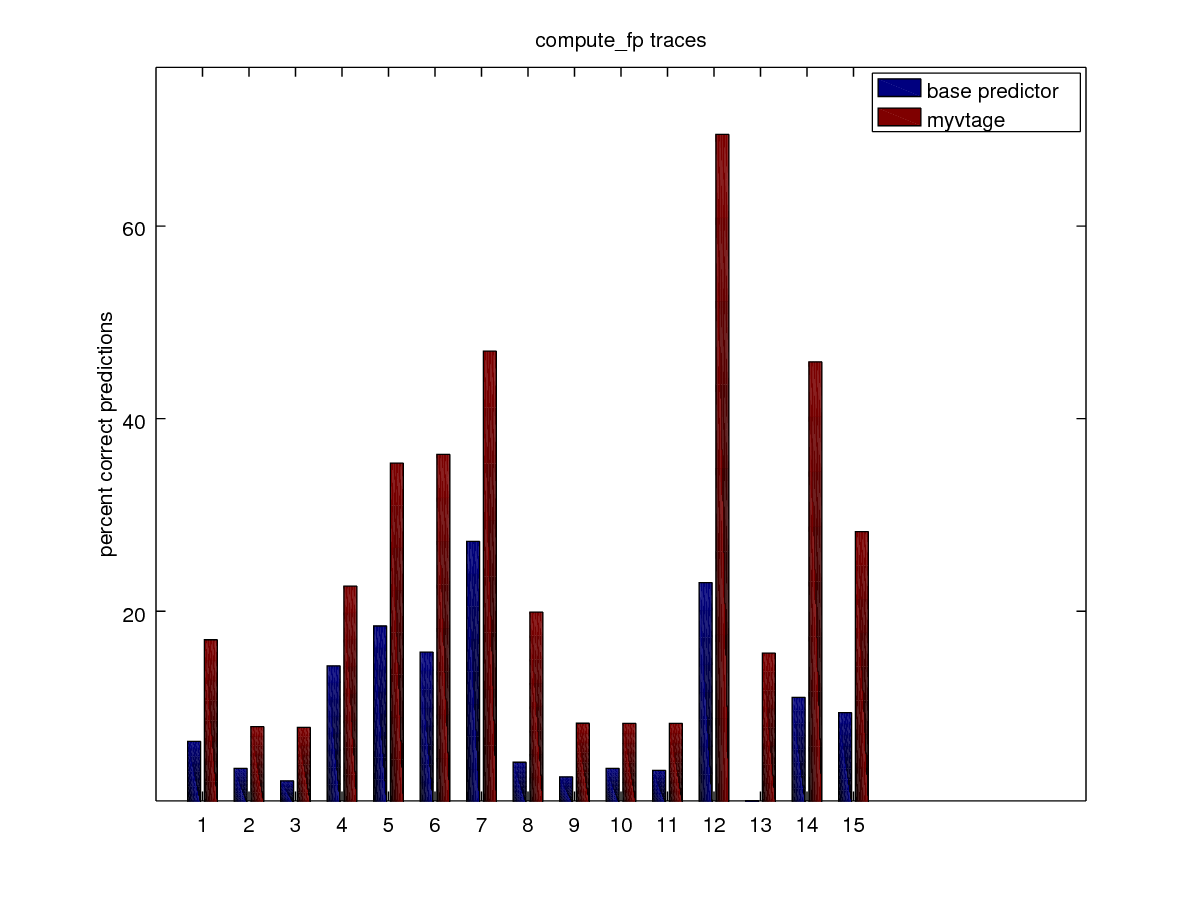
\includegraphics[width=0.75\textwidth]{compute_fptraces1.png}
		\caption{compute\_fp traces. base avg = 9.7653, myvtage avg = 25.2433}
		\label{fig:computefp1}
	\end{figure}
	\begin{figure}[p]
		\centering
		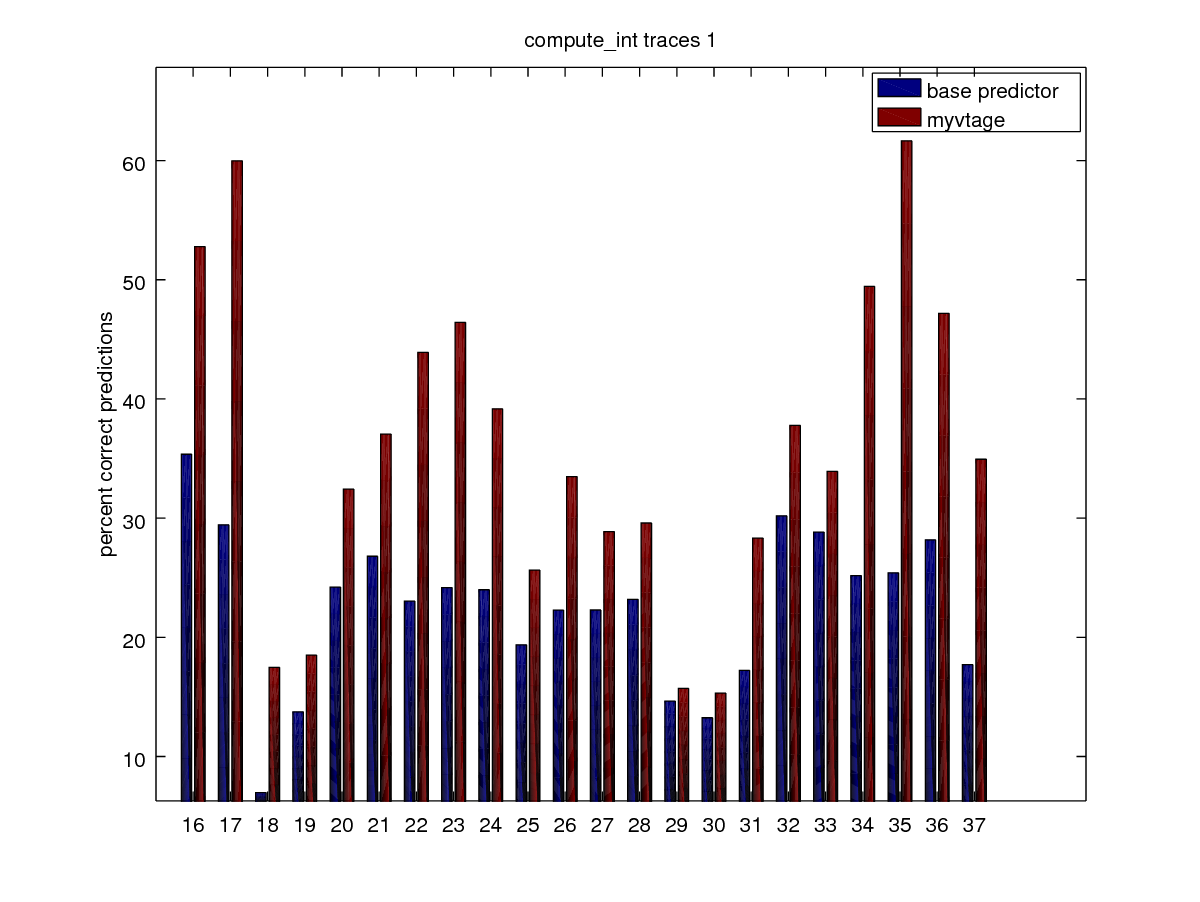
\includegraphics[width=0.75\textwidth]{compute_inttraces1.png}
		\caption{compute\_int traces 1 (traces split into 2 groups to more easily view). base avg = 22.588, myvtage avg = 35.414}
		\label{fig:computeint1}
	\end{figure}
	\begin{figure}[p]
		\centering
		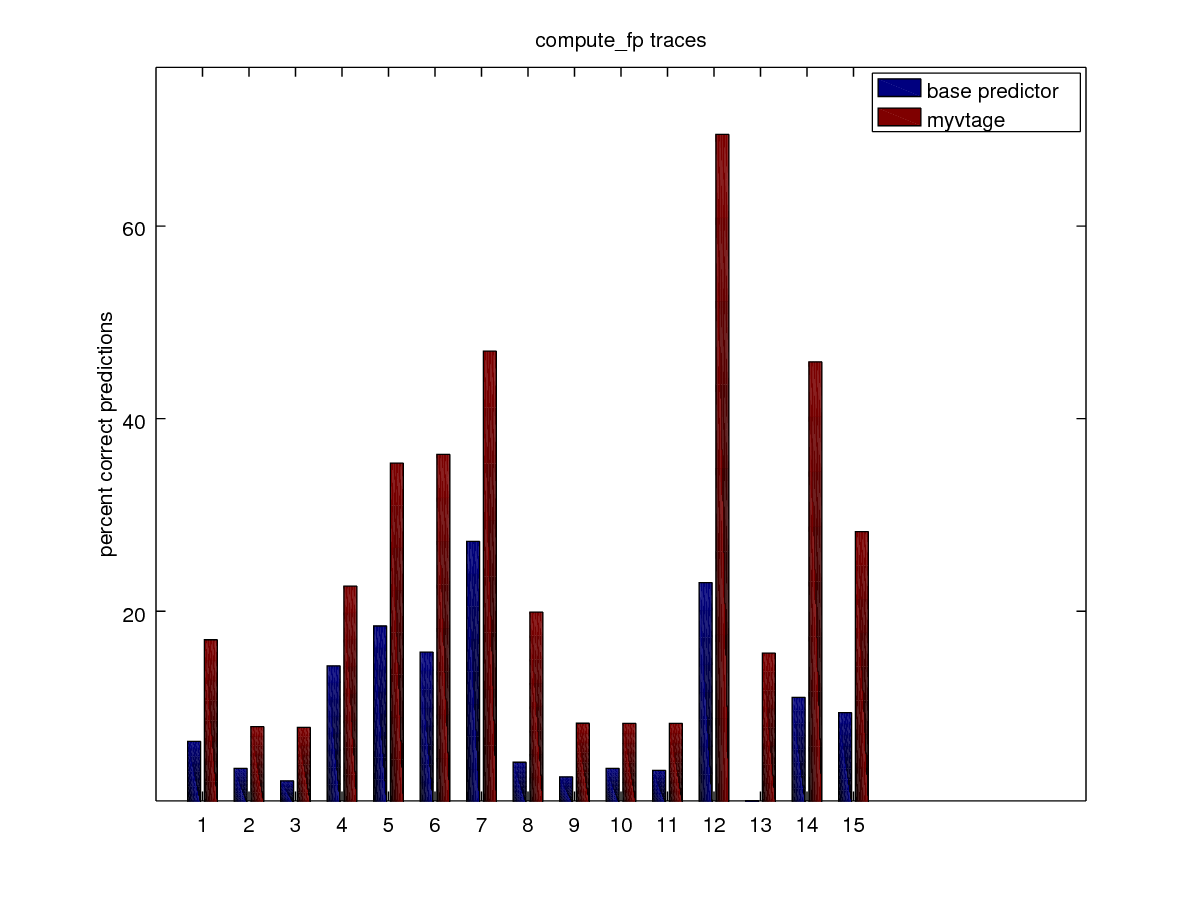
\includegraphics[width=0.75\textwidth]{compute_inttraces2.png}
		\caption{compute\_int traces 2}
		\label{fig:computeint2}
	\end{figure}
	\begin{figure}[p]
		\centering
		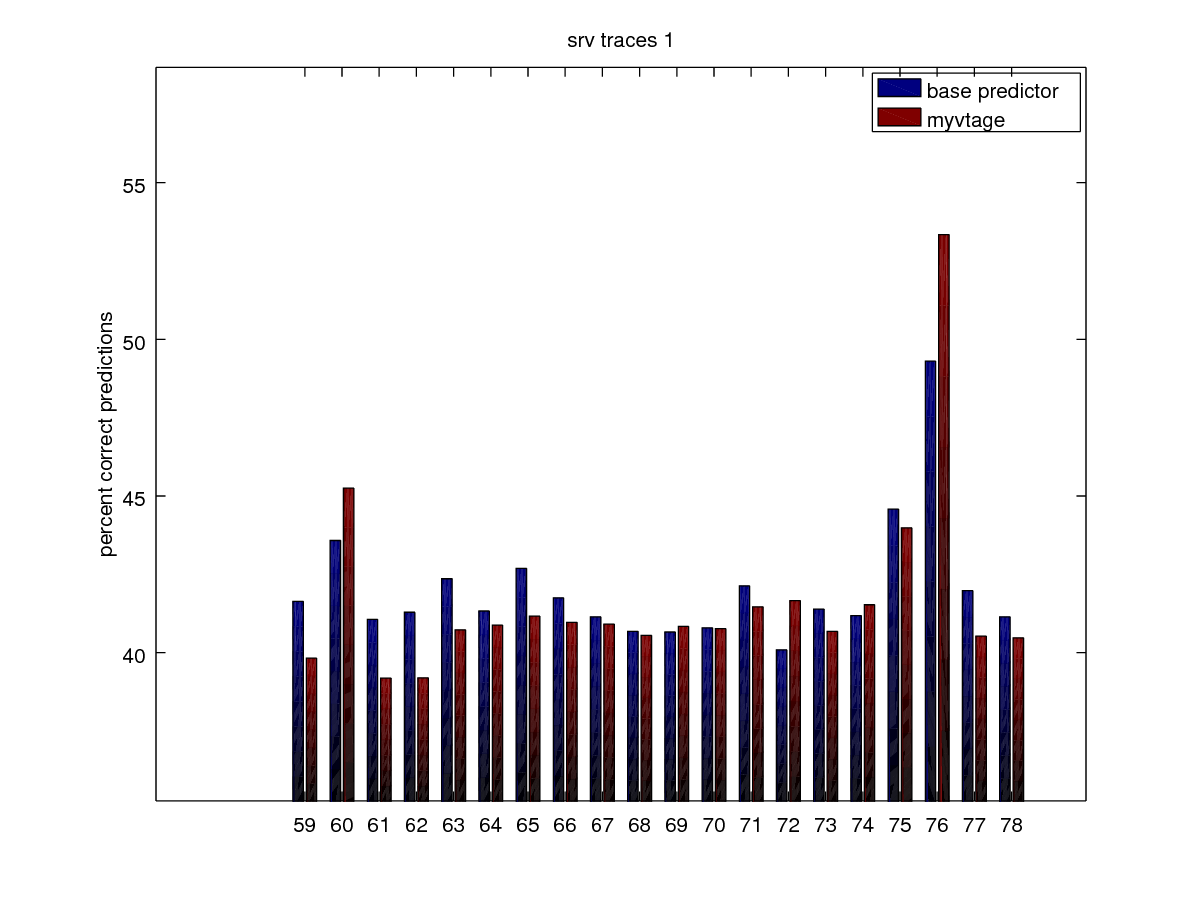
\includegraphics[width=0.75\textwidth]{srvtraces1.png}
		\caption{srv traces 1 (traces split into 4 groups to more easily view). base avg = 28.731, myvtage avg = 31.144}
		\label{fig:srv1}
	\end{figure}
	\begin{figure}[p]
		\centering
		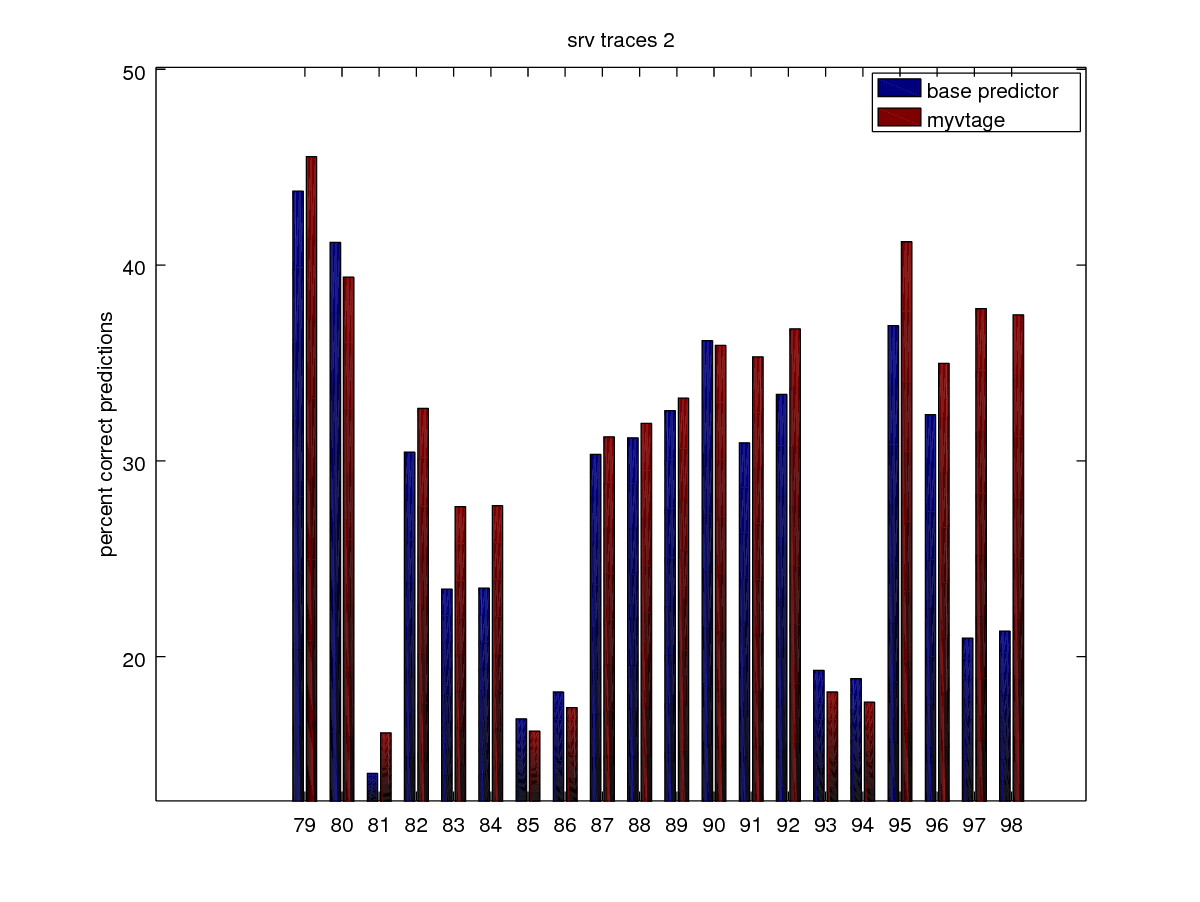
\includegraphics[width=0.75\textwidth]{srvtraces2.png}
		\caption{srv traces 2}
		\label{fig:srv2}
	\end{figure}
	\begin{figure}[p]
		\centering
		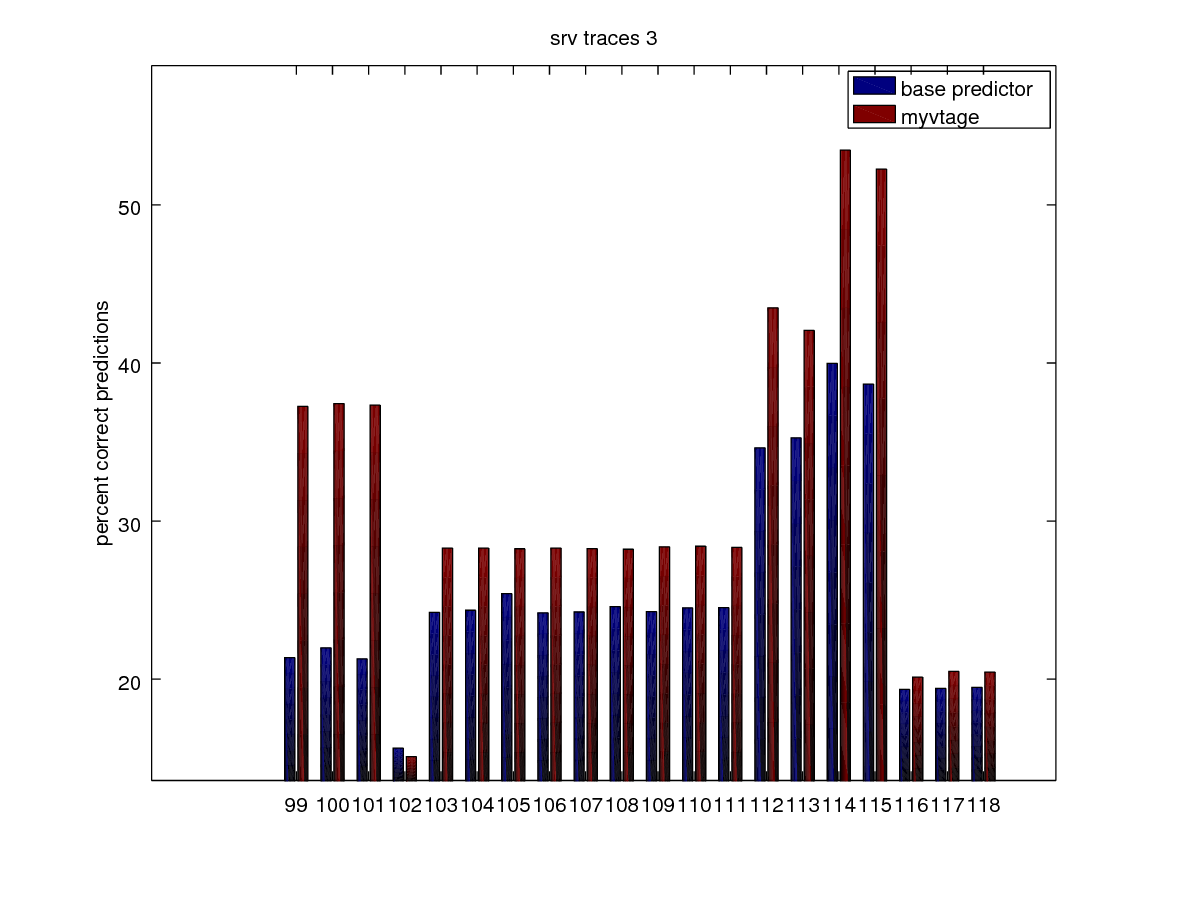
\includegraphics[width=0.75\textwidth]{srvtraces3.png}
		\caption{srv traces 3.}
		\label{fig:srv3}
	\end{figure}
	\begin{figure}[p]
		\centering
		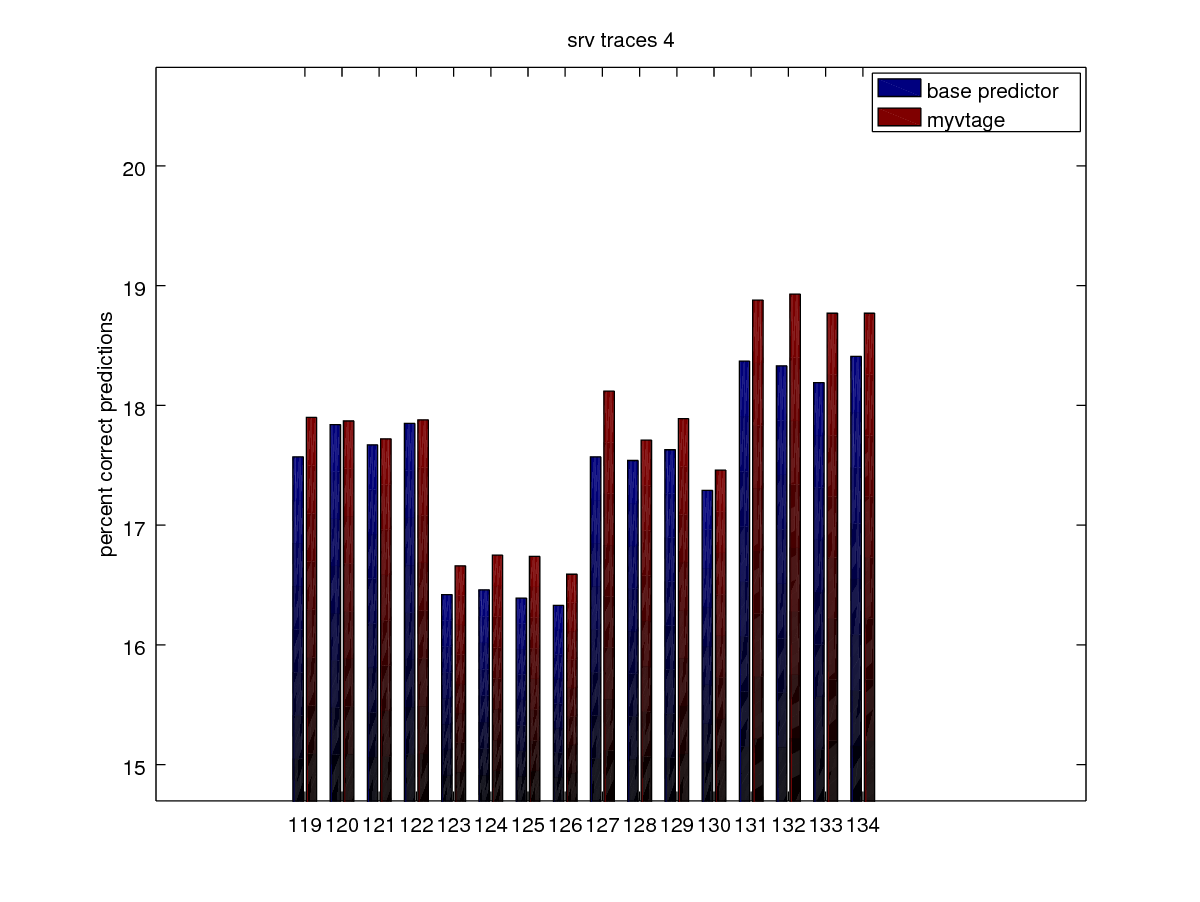
\includegraphics[width=0.75\textwidth]{srvtraces4.png}
		\caption{srv traces 4.}
		\label{fig:srv4}
	\end{figure}
\end{document}
